\documentclass[12pt]{exam}
\usepackage{amsmath}
\usepackage{amssymb}
\usepackage{amsthm}
\usepackage{tikz}
\usepackage{mathtools}
\usepackage{graphicx}
\usepackage{wrapfig}

\usepackage{bm} %bold symbols
\usepackage{hyperref} %add links

%%%%%%%%%%%%%%%%%%%%%%%%%
% 	Define vars here 	%
%%%%%%%%%%%%%%%%%%%%%%%%%

\def\hwName{Homework Set}
\author{Zhengyu James Pan} %use like \@author
\def\email{jzpan@umich.edu}
\makeatletter

\begin{document}
%Header
\pagestyle{head}
\firstpageheader{}{}{}
\header{MATH 215}{\hwName}{\thepage}

%Solution formatting
\printanswers
\unframedsolutions

%Top matter
{\parindent0in
\begin{center}
	\bf MATH 215 FALL 2023\\
	\bf \hwName \\
	\@author\ (\href{mailto:\email}{\email})
\end{center}
}

\begin{questions}
%1
\question The surface S defined by $x^2 + 2xy - y^2 - zy - z^2 - 3xz = 100$ is a hyperboloid of two sheets. Find the point on $S$ with smallest positive x-coordinate.
%2
\question In this question we will look at a function with multiple constraints and see that sometimes the constraints
are more restrictive than we think. Let $f (x, y) = x^2 + y^2 - 2x - 4y$, and let A be the region defined by
$x \geq 0$, $0 \leq y \leq 5$, and $y \geq x$.
    \begin{parts}
        \part Find the absolute maximum and minimum values of $f$ on the region $A$. It is a good idea to draw $A$ for this problem.
            \begin{solution}
                The gradient of f is $\nabla f(x, y) = \langle 2x - 2, 2y - 4 \rangle$ 
            \end{solution}
        \part Now add a second restriction. Let $C$ be the circle of radius 4 centered at the origin, and find the extremal values of $f$ restricted to the set of points that lie in both $A$ and $C$. Note that the region $A$ contains the interior of the triangle, while $C$ is only the boundary of the circle. It is definitely a good idea to draw both $A$ and $C$ for this part.
            \begin{solution}This region is equivalent to the arc of the circle where $0 \leq x \leq y$.\\
                \tikzset{every picture/.style={line width=0.75pt}} %set default line width to 0.75pt        

                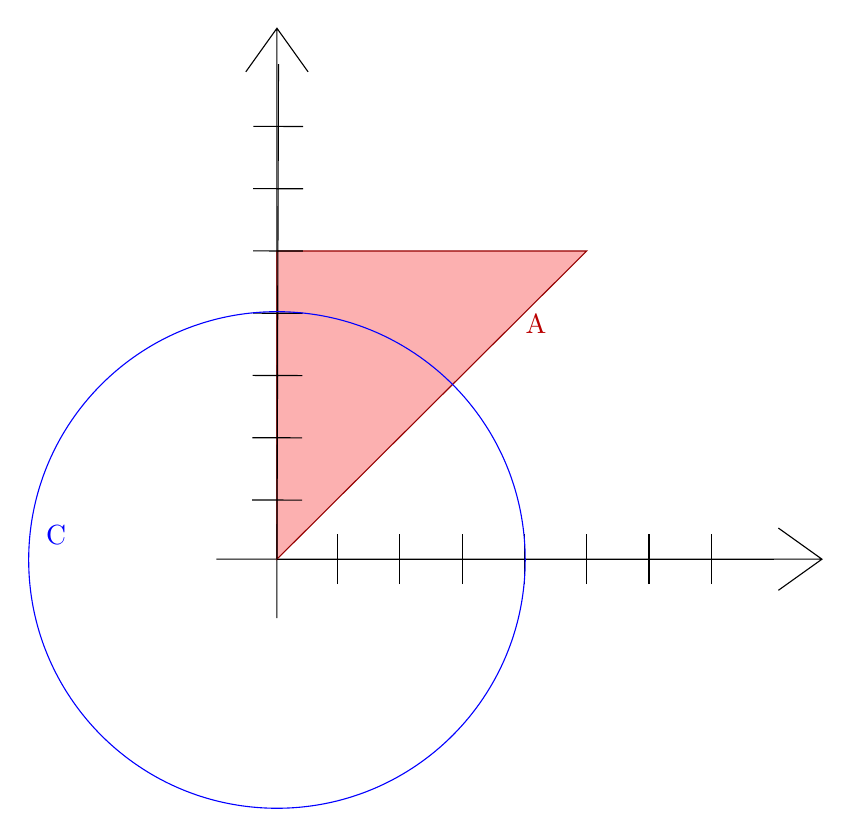
\begin{tikzpicture}[x=0.75pt,y=0.75pt,yscale=-3,xscale=3]
                %uncomment if require: \path (0,300); %set diagram left start at 0, and has height of 300
                
                %Shape: Axis 2D [id:dp8217938239242988] 
                \draw  (290.77,239.75) -- (388.03,239.75)(300.5,154.48) -- (300.5,249.23) (381.03,234.75) -- (388.03,239.75) -- (381.03,244.75) (295.5,161.48) -- (300.5,154.48) -- (305.5,161.48)  ;
                %Shape: Right Triangle [id:dp1989773638582364] 
                \draw  [color={rgb, 255:red, 150; green, 0; blue, 0 }  ,draw opacity=1 ][fill={rgb, 255:red, 245; green, 0; blue, 0 }  ,fill opacity=0.31 ] (300.5,239.75) -- (350.25,190.25) -- (300.5,190.25) -- cycle ;
                %Straight Lines [id:da2778595943944473] 
                \draw    (380.25,239.75) -- (326,239.75) -- (300.5,239.75) (370.25,243.75) -- (370.25,235.75)(360.25,243.75) -- (360.25,235.75)(350.25,243.75) -- (350.25,235.75)(340.25,243.75) -- (340.25,235.75)(330.25,243.75) -- (330.25,235.75)(320.25,243.75) -- (320.25,235.75)(310.25,243.75) -- (310.25,235.75) ;
                %Straight Lines [id:da6147731998804034] 
                \draw    (300.75,160.25) -- (300.5,239.75) (304.72,170.26) -- (296.72,170.24)(304.69,180.26) -- (296.69,180.24)(304.66,190.26) -- (296.66,190.24)(304.62,200.26) -- (296.62,200.24)(304.59,210.26) -- (296.59,210.24)(304.56,220.26) -- (296.56,220.24)(304.53,230.26) -- (296.53,230.24) ;
                %Shape: Circle [id:dp1717765113509926] 
                \draw  [color={rgb, 255:red, 3; green, 0; blue, 255 }  ,draw opacity=1 ] (260.63,240) .. controls (260.56,217.98) and (278.36,200.07) .. (300.38,200) .. controls (322.4,199.93) and (340.31,217.73) .. (340.37,239.75) .. controls (340.44,261.77) and (322.65,279.68) .. (300.63,279.75) .. controls (278.61,279.82) and (260.7,262.02) .. (260.63,240) -- cycle ;
                
                % Text Node
                \draw (263,234) node [anchor=north west][inner sep=0.75pt]  [xscale=1,yscale=1] [align=left] {\textcolor[rgb]{0,0,1}{C}};
                % Text Node
                \draw (340,200) node [anchor=north west][inner sep=0.75pt]  [xscale=1,yscale=1] [align=left] {\textcolor[rgb]{0.73,0,0}{A}};
                
                \end{tikzpicture}\\
                
                This circle is defined by $x^2 + y^2 = 16$. The gradient of this equation is $\langle 2x, 2y \rangle$. So, we create a system using Lagrange multipliers.
                \begin{gather*}
                    \begin{cases*}
                        2x - 2 = \lambda 2x \\
                        2y - 4 = \lambda 2y \\
                        x^2 + y^2 = 16 \\
                        x \geq 0 \\
                        y \geq x
                    \end{cases*} \\
                    y = \sqrt{16 - x^2} \\\\
                    2\sqrt{16 - x^2} - 4 = 2\lambda \sqrt{16 - x^2} \\
                    \lambda = 1 - \frac{2}{\sqrt{16 - x^2}} \\
                    2x - 2 = 2\left(1 - \frac{2}{\sqrt{16 - x^2}}\right)x \\\\
                    1 - \frac{1}{x} = 1 - \frac{2}{\sqrt{16 - x^2}} \\
                    \frac{1}{x} = \frac{2}{\sqrt{16 - x^2}} \\
                    x^2 = 4 - \frac{x^2}{4} \\
                    \frac{5x^2}{4} = 4 \\
                    x = \frac{4}{\sqrt{5}} \\
                    y = \frac{8}{\sqrt{5}}
                \end{gather*}
                Since $x$ and $y$ must both be positive, this is the only critical point in this region. Thus, we check this point and the boundary points for extremal values.
                \begin{gather*}
                    \boxed{f(\frac{4}{\sqrt{5}}, \frac{8}{\sqrt{5}}) = 16 - \frac{40}{\sqrt{5}} \approx -1.88854382} \\
                    \boxed{f(0, 4) = 0} \\
                    f(2\sqrt{2}, 2\sqrt{2}) = 16 - 12\sqrt{2} \approx -0.9705627485 \tag*{\qed}
                \end{gather*}
            \end{solution}
        \part Repeat the previous part of the problem, except let the radius of $C$ be $\sqrt{50}$.
            \begin{solution}
                We can repeat the same process as the last problem.
                \begin{gather*}
                    \begin{cases*}
                        2x - 2 = \lambda 2x \\
                        2y - 4 = \lambda 2y \\
                        x^2 + y^2 = 50 \\
                        x \geq 0 \\
                        y \geq x
                    \end{cases*} \\
                    y = \sqrt{50 - x^2} \\\\
                    2\sqrt{50 - x^2} - 4 = 2\lambda \sqrt{50 - x^2} \\
                    \lambda = 1 - \frac{2}{\sqrt{50 - x^2}} \\
                    2x - 2 = 2\left(1 - \frac{2}{\sqrt{50 - x^2}}\right)x \\\\
                    1 - \frac{1}{x} = 1 - \frac{2}{\sqrt{50 - x^2}} \\
                    \frac{1}{x} = \frac{2}{\sqrt{50 - x^2}} \\
                    x^2 = \frac{50}{4} - \frac{x^2}{4} \\
                    5x^2 = 50 \\
                    x = \sqrt{10} \\
                    y = 2\sqrt{10}
                \end{gather*}
                Since $x$ and $y$ must both be positive, this is the only critical point in this region. Thus, we check this point and the boundary points for extremal values.
                \begin{gather*}
                    \boxed{f(\sqrt{10}, 2\sqrt{10}) = 50 - 10\sqrt{10} \approx 18.3772234} \\
                    \boxed{f(0, \sqrt{50}) = 50 - 8\sqrt{10} \approx{21.71572875}} \\
                    f(5, 5) = 20 \tag*{\qed}
                \end{gather*}
            \end{solution}
    \end{parts}
%3
\question In this question we will look at a function with multiple constraints and see that sometimes the constraints are secretly not as bad as we thought. Find the extreme values for the function $zx + 2xy$ subject to the two constraints $y + z = 1$ and $x^2 + y^2 = 1$. This problem may be easier than it appears, and it is worth some time to think hard about it before you start computing.
    \begin{solution}
        %We begin by finding the intersection of the constraints. The first constraint is a plane not parallel to the $xy$ plane, and the first constraint is cylinder based on a circle within the $xy$ plane. 
        The gradient of the function is $\nabla f(x, y, z) = \langle z + 2y, 2x, x \rangle$. The gradients of the constraints are $\langle 0, 1, 1 \rangle$ and $\langle 2x, 2y, 0 \rangle$ respectively.
        We find a system from Lagrange multipliers with these constraints.
        \begin{gather*}
            \begin{cases*}
                z + 2y = \lambda_2 2x \\
                2x = \lambda_1 + \lambda_2 2y \\
                x = \lambda_1 \\
                y + z = 1 \\
                x^2 + y^2 = 1
            \end{cases*}\\
            \begin{cases*}
                z + 2y = \lambda_2 2x \\
                x = \lambda_2 2y \\
                y + z = 1 \\
                x^2 + y^2 = 1
            \end{cases*} \\
            z + 2y = \lambda_2^2 4y \\
            1 + y = \lambda_2^2 4y \\
            \pm \sqrt{\frac{1 + y}{4y}} = \lambda_2 \\
            (\lambda_2 2y)^2 + y^2 = 1 \\
            \frac{1 + y}{4y}4y^2 + y^2 = 1 \\
            y + y^2 + y^2 = 1\\
            (2y-1)(y+1) = 0 \\
            y = -1, \frac{1}{2} \\
            x = 0, \pm \frac{\sqrt{3}}{2} \\
            z = 2, \frac{1}{2}\\
            \\
            \boxed {f(-1, 0, 2) = -2} \\
            f(-\frac{\sqrt{3}}{2}, \frac{1}{2}, \frac{1}{2}) = -\frac{3\sqrt{3}}{4} \approx -1.299038106 \\
            \boxed {\frac{\sqrt{3}}{2}, f(\frac{1}{2}, \frac{1}{2}) = \frac{3\sqrt{3}}{4} \approx 1.299038106}
        \end{gather*}
    \end{solution}
%4
\question In this question we will look at a function with multiple constraints and see that the worst part is the
algebra. Find the extreme values of $f (x, y, z) = x^2 + y^2 + z^2$ subject to the constraints $x - y = 1$ and $y^2 - z^2 = 1$.
%5
\question Calculate the following iterated integrals:
    \begin{parts}
        \part \[\int_{0}^{1}\int_{y}^{1}ye^{x^3}\, dx\, dy\]
        \part \[\int_{0}^{2}\int_{y/2}^{1}y\cos(x^3 - 1)\, dx\, dy\]
    \end{parts}
%6
\question In evaluating a double integral over a region $D$, a sum of iterated integrals was obtained as follows:
\[ \int_{D}f(x, y)\,dA=\int_{-9}^{0}\int_{-2}^{1-\sqrt{-y}}f(x, y)\, dx\, dy\]
Sketch the region $D$ and express the double integral as an iterated integral with reversed order of
integration.
%7
\question Let $D = [-2, 2] \times [-1, 1]$. Show that
\[ \frac{4}{3} \leq \int_{}^{} \int_{D}^{} \left(\frac{xe^{10y^2}}{1+ x^8 + y^2} + \frac{1}{1 + x^2 + y^4} \right)\, dA \leq 8\] 
Hint: It is easier to estimate these two integrals separately. Also note that the bounds I have provided may not be the tightest possible bounds -- it is likely you can do better with a little thought.
    \begin{solution}
        Let $f(x, y) = \frac{xe^{10y^2}}{1+ x^8 + y^2}$ and $g(x, y) = \frac{1}{1 + x^2 + y^4}$. We will evaluate these functions separately.\\\\
        We can observe that $z = f(x, y)$ is even when we fix $x$ and vary $y$, and odd when we fix $y$ and vary $x$. Thus, since the bounds of the integral are symmetrical accross $x$, the integral of the region with $x>0$ will be the negative of the integral of the region with $x<0$. (The value at 0 is 0.) Therefore, the total value of the integral of $f$ is 0.\\\\
        Since the denominator of $g(x, y)$ can only increase, its maximum must be when the denominator is minimized, giving a maximum value of 1. It will have a minimum when the denominator is 0, which is $\frac{1}{6}$ in the integration bounds. Thus, the minimum value the integral can have is product of the area of the region of integration with the minimum, and similarly for the max. This grants a minimum of $\frac{4}{3}$ and a maximum of 8 for the integral of $g$.\\\\
        Putting the bounds of these two integrals together, 
        \[ \boxed{ \frac{4}{3} \leq \int_{}^{} \int_{D}^{} \frac{xe^{10y^2}}{1+ x^8 + y^2}\, dA + \int_{}^{} \int_{D}^{} \frac{1}{1 + x^2 + y^4}\, dA \leq 8 } \tag*{\qed}\] 
    \end{solution}
%8
\question  In this question we will approximate an integral through a Riemann sum. Specifically, we will adapt a two-dimensional version of the trapezoid rule. Suppose you have been tasked to estimate the volume of
a swimming pool with square base (denoted by $R$) with side length 12 feet. The depth of the pool in feet is measured every 3 feet (i.e. once at position 0, once at position 3 feet, once at position 6 feet, so
forth and so on), and this data is presented in the table below. Estimate the volume of the pool as the average of 4 Riemann sums, where each Riemann sum uses a subdivision of the regions into 16 squares
with a different corner as a sample point. The data is given as:
\begin{center}
    \includegraphics*[scale=0.7]{images/06-data.png}
\end{center}


\end{questions}
\end{document}